\documentclass[ddcfooter,nosectionnum]{tudbeamer}
\usepackage{german}
\usepackage{graphicx}

\usepackage{listings}
\usepackage{setspace}
\usepackage{array}
\usepackage{wrapfig}




\usepackage{fontspec}
\usepackage{xltxtra}
\setmainfont{Ubuntu}
\setmonofont{Courier}
\setromanfont{Ubuntu}
\setsansfont{Ubuntu}

\begin{document}

\einrichtung{Fakultät Informatik\hspace{6cm} Institut für Systemarchitektur}
\title[Speicherverwaltung in Linux]{Speicherverwaltung in Linux}
\subtitle{Proseminar Betriebssysteme}
\author{Rebecca Kratsch}

\date{10.05.2013}

\maketitle
	

\begin{frame}
    \frametitle{Inhalt}
	\tableofcontents
\end{frame}



\section{Grundlagen}
\begin{frame}
	\frametitle{Grundlagen}
    \framesubtitle {Gliederung eines Linux-Prozess-Adressraumes }
	
		\begin{table}[ht]
		\centering
			\begin{tabular}{*{2}{m{0.5\textwidth}}}
			\includegraphics[width = 3cm]{folie_1.eps} &
			\begin{itemize}
		 		\item Stack:  
				\begin{itemize}
					\item Umgebungsvariablen, Kommandozeile, lokale Variablen
					\item veränderbar
				\end{itemize}  	
				\item Datensegment:  
				\begin{itemize}
					\item initialisierte Daten    
					\item uninitialisierte Daten ( Verweis auf Zeropage)
				\end{itemize}
				\item Textsegment: 
				\begin{itemize}
					\item Maschinenbefehle
					\item nur lesender Zugriff
					\item keine Größenänderung mögl. 
				\end{itemize}
    		\end{itemize}
%&\includegraphics[width=4cm]{folie_1.eps}
			\end{tabular}
			\label{tab:gt}
		\end{table}
\end{frame}


\begin{frame} 
    \frametitle{Grundlagen}
    \framesubtitle{Memory-Mapped-Dateien}
    \begin{figure}[p]  
    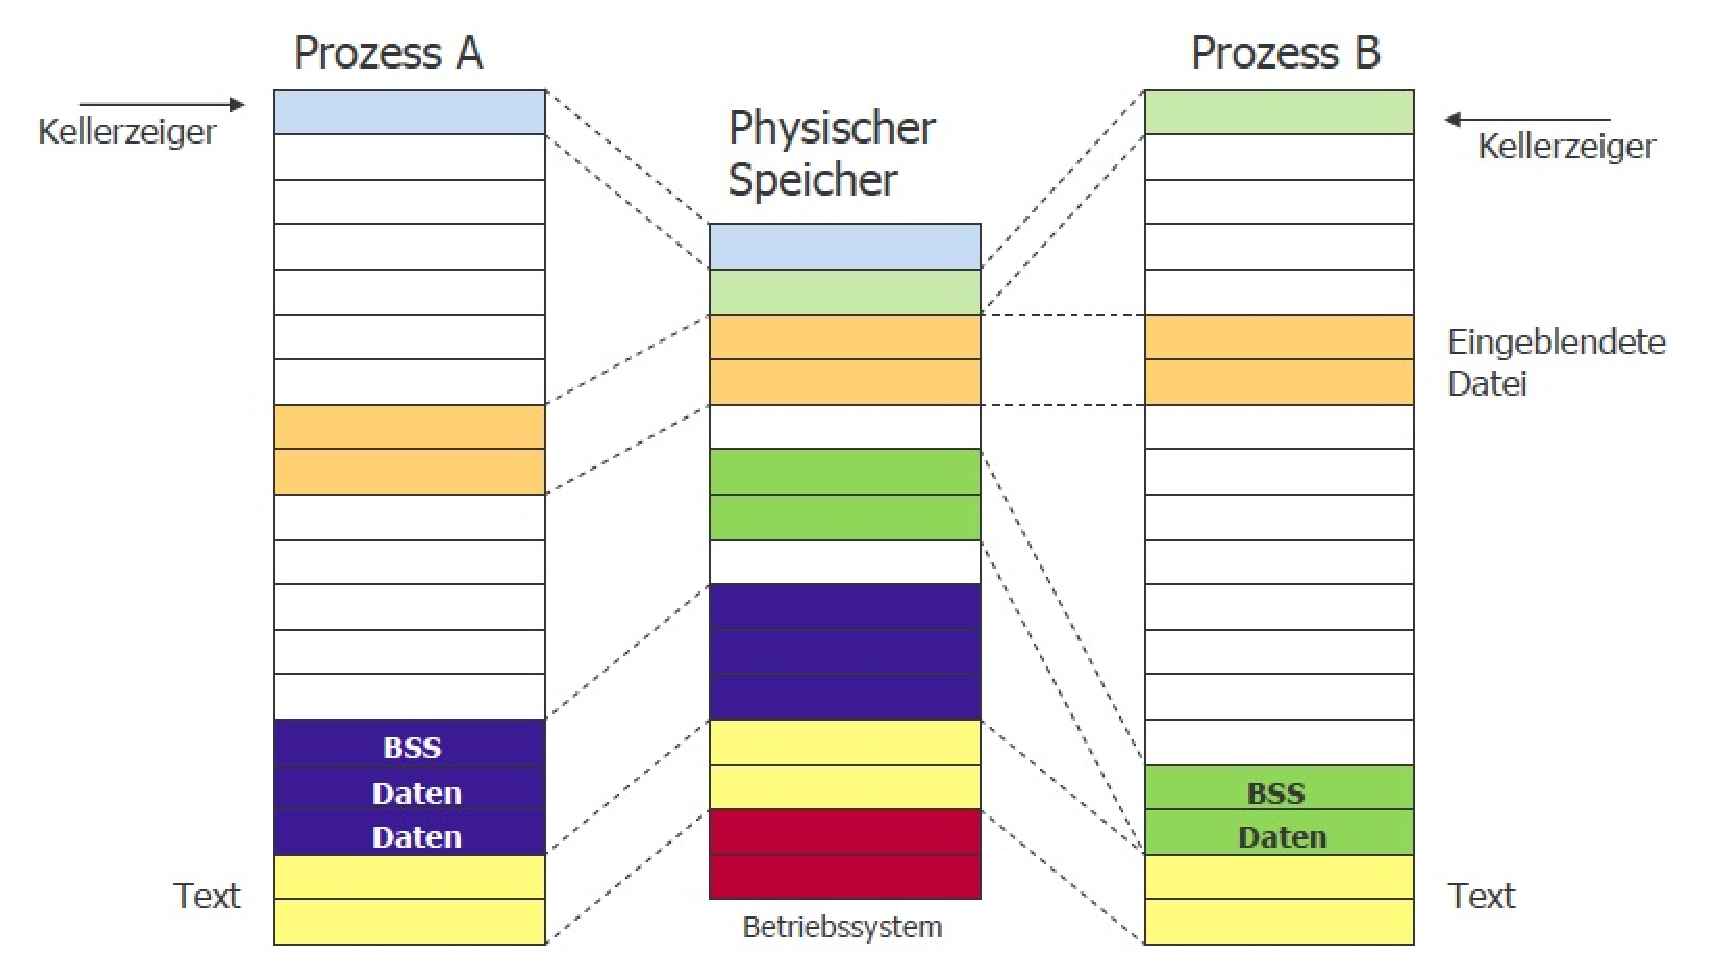
\includegraphics[width=9cm]{segmente.eps}
    \caption{Kao,O.; Vorlesung Betriebssysteme; Universität Paderborn; 2005)} 
     \end{figure}
\end{frame}

\section{Implementierung der Speicherverwaltung}
%\begin{frame}
%    \frametitle{was ihr wollt}
%   
%   \begin{itemize}
%         		\item 3 Speicherzonen: ( Grafik noch einfügen)
%
%		\begin{itemize}
%			\item 1 Zone_DMA
%			\item 2 Zone_Normal
%			\item 3 Zone_Highmen
%		\end{itemize}
%   	\end{itemize} 
%\end{frame}

\begin{frame}
    \frametitle{noch unklar}
   
   \begin{itemize}
         		\item Seitendeskriptor
		\item Zonendeskriptor
		\item Knotendeskriptor\\
			
			----eventuell mit Grafik--
			
	
   	\end{itemize} 

   
       
\end{frame}



%\section{Systemaufrufe}
%\begin{frame}
%    \frametitle{Systemaufrufe zur Speicherverwaltung}
%   
%    \begin{center}
%   	 \begin{tabular}{ | l |m{5cm} |}
%   	 \hline
%   	 Systemaufruf & Beschreibung \\ \hline
%    	s= brk(addr) & Datensegmentgröße ändern \\ \hline
%    	a = mmap(addr, len, prot, flags, fd, offset)&  Datei einblenden \\ \hline
%    	s = munmap(addr, len)  & Dateieinblendung beenden\\ \hline
%    	\end{tabular}
%    \end{center} 
%       
%\end{frame}





\section{virtueller Speicher}
\begin{frame}
    \frametitle{Virtueller Adressraum}
    \begin{itemize}
         \item   Unterteilung in homogene, zusammenhängende, an Seitengrenzen ausgerichtete 			Regionen
         \item fixe Seitengröße, erweiterbar durch PAE
        
     \end{itemize}
    
\end{frame}


\section{virtueller Speicher}
\begin{frame}
    \frametitle{Virtuellen Adressraum}
    \begin{itemize}
    	    \item Beschreibung jedes Kernbereichs mit \texttt{vm\_area\_struct}-Eintrag 
   		\begin{itemize}
			 \item sortiert und zusammengefasst nach virtueller Adresse\\
			\item enthält Eigenschaften (Schutzrechte...)
			--> Realisiserung Copy- on-Write
			\item Angaben über Hintergrundspeicher
    			\item Zugriff auf alle Elemenete eines Adressraumes via Speicher-Deskriptor
			\begin{itemize}
				\item verkettete Liste
				\item binärer Rot-Schwarz-Baum
			\end{itemize}
   		\end{itemize} 
	\end{itemize}
    
\end{frame}

\begin{frame}
    \frametitle{Virtueller Adressraumes}
    \framesubtitle {Paging in Linux}
    \begin{itemize}
         \item  Grundeinheit: Seite
         \item Grundidee / Definition Paging: \\
        \begin{quote}
         „Paging ist ein Speicherverwaltungsverfahren, das auf der Strukturierung  des virtuellen Speichers 	in Seiten und der Strukturierung des realen Speichers in Seitenrahmen beruht.“
         \footnote{EHSES, E. u.a. : Betriebssysteme- Ein Lehrbuch mit Übungen zur Systemrogrammierung in UNIX/Linux. 3. Aufl. München: Pearson Studium Verlag, 2005, S.294}
	\end{quote}
 	
	
    
    
     \end{itemize}
    
\end{frame}


\begin{frame}
    \frametitle{Virtueller Adressraum}
    \framesubtitle {Paging in Linux}
    \begin{itemize}
         \item Nutzung 4-stufiger Seitentabellen in Linux\\
         --------Grafik überarbeiten ----------
	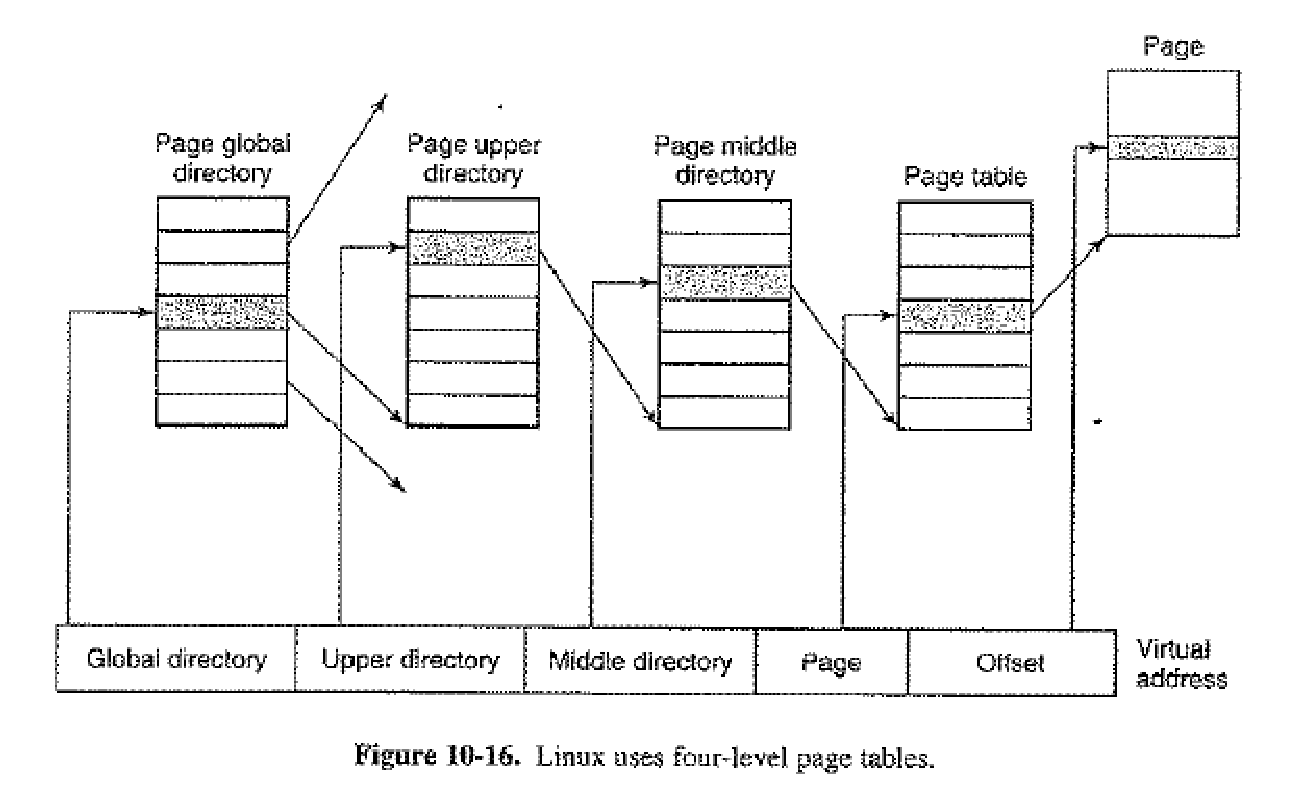
\includegraphics[width=6cm]{Seitentab.eps} 		
    
    
     \end{itemize}
    
\end{frame}


\begin{frame}
 
    \frametitle {Virtueller Adressraum}
    
    \framesubtitle {Paging in Linux}
    \begin{itemize}
         \item  Grundeinheit: Seite
         \item Grundidee / Definition Paging: \\
        \begin{quote}
         „Paging ist ein Speicherverwaltungsverfahren, das auf der Strukturierung  des virtuellen Speichers 	in Seiten und der Strukturierung des realen Speichers in Seitenrahmen beruht.“
     	 \end{quote}
 	 \item Nutzung 4-stufiger Seitentabellen in Linux
	 \item Realisierung sowohl durch kern als auch durch Page-Daemon
	 \item Demand - Paging - System unter Nutzung des Swap-Bereiches
	 \begin{itemize}
	 	\item Auslagerungspartitionen 
		\item Auslagerungsdateien
	\end{itemize}
    
    
     \end{itemize}
    
\end{frame}

\begin{frame}
	\frametitle{Virtueller Adressraum}\
	\framesubtitle {Der Seitenersetzungsalgorithmus}
 	\begin{itemize}
		\item per Page Frame Reclaiming Algorithmus
		\item Unterscheidung von vier Seitenarten:
	\end{itemize}	
		
		\begin{center}
		{\tiny
		\begin{tabular}{ l l }
 			 unreclaimable :&  reserviert/gesperrt/nicht auslagerbar \\
  			 swappable:       &  zurück auf Swap bzw Auslagerungspartition vor Neuanforderung\\
 			 syncable:		 &  zurück auf Platte, falls verändert\\
			 discardable:      & sofort anforderbar\\
		\end{tabular}
		}
		\end{center}
		
		zu beenden

			
    
\end{frame}



\section{Zusammenfassung}
\begin{frame}
    \frametitle{Zusammenfassung}
    \begin{itemize}
         \item   
    
    
    
     \end{itemize}
    
\end{frame}


\section{Literatur}
\begin{frame}
    \frametitle{Literatur}
    \begin{itemize}
         \item  Moderne Betriebssysteme \\
        		Andrew S. Tanenbaum - 2010
	\item	 UNIX - Wie funktioniert das Betriebssystem? \\
		Maurice J. Bach - 1991
	\item Betriebssysteme\\
		EIn Lehrbuch mit Übungen zur Systemprogrammierung in UNIX/ Linux \\
		E.Ehses, L. Köhler, P. Riemer, H. Stenzel, F. Victor - 2010	
    \end{itemize}
    
\end{frame}

\end{document}






